\chapter{Task 6}
\begin{figure}[hbt]	
\label{Task6}
  \centering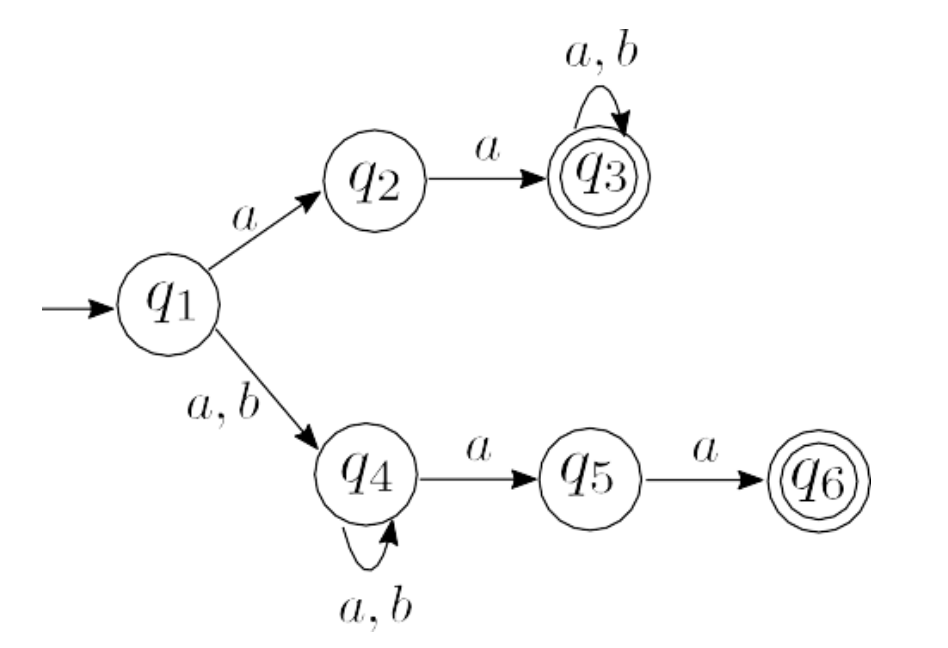
\includegraphics[width=\textwidth]{Immagini/fsm_task6.png}
  \caption{Task6}
\end{figure}
The Figure shown above, represent a NFA that accepts the language composed by the alphabet ${a,b, \epsilon}$ where all strings accepted are constructed as follows:
\begin{itemize}
	\item if the string doesn't start with a $b$ then all the strings that end with $aab$ are accepted.
	\item if the string starts with a $b$ then all the strings that end with $aa$ are accepeted.
\end{itemize}
The reason being the fact that NFA when given an input that would be processed by multiple state, like in this case the input $a$ would be accepted simultaneously by state $q_2$ and $q_4$; the machine would be split up in two different machine and if even one of the multiple machine in which an NFA would split accept the given input then, the input is accepted. In the case discussed, if the $a$ input would go to state $q_2$ then the string accepted would be the one that end with "$aab$". If the we were taking in consideration the case in which the $a$ in input would be accepted by the $q_4$ state then the string accepted would be the one that end with "$aa$".\cite{Sipser:2006aa}
